\documentclass{article}
\usepackage{tikz}
\usetikzlibrary{folding}
\begin{document}
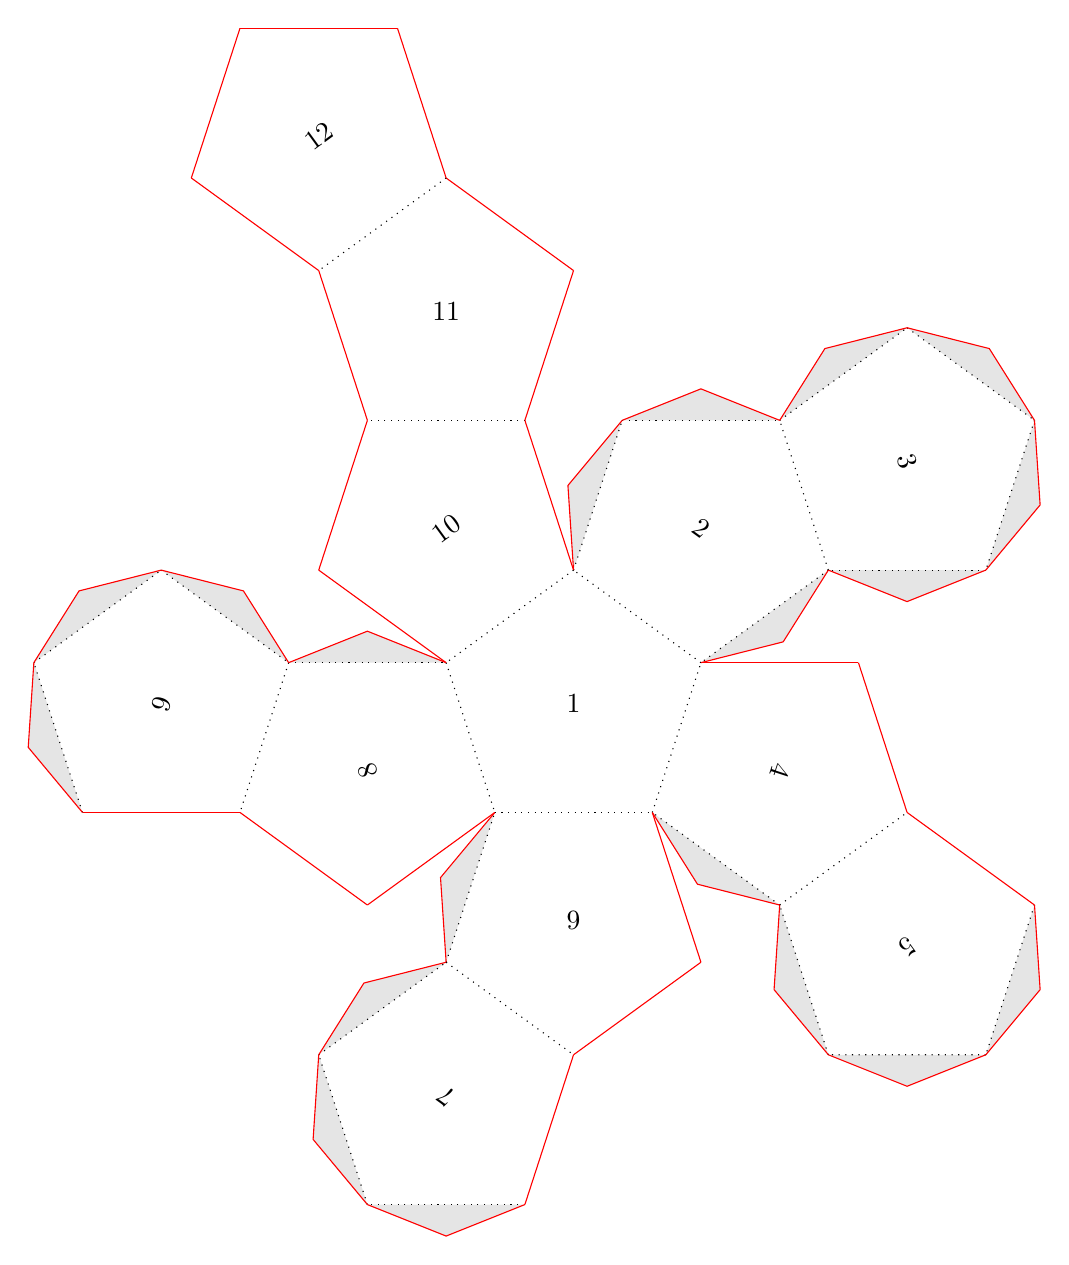
\begin{tikzpicture}[transform shape,every cut/.style=red,every fold/.style=dotted,every ear/.style={fill,gray!20}]
	\tikzfoldingdodecahedron
	[folding line length=20mm,numbered faces];
\end{tikzpicture}
\clearpage
\begin{tikzpicture}[transform shape,every cut/.style=red,every fold/.style=dotted]
	\tikzfoldingalternatedodecahedron
	[folding line length=20mm,numbered faces];
\end{tikzpicture}
\clearpage
\begin{tikzpicture}[transform shape,every cut/.style=red,every fold/.style=dotted]
	\tikzfoldingtetrahedron
	[folding line length=40mm,numbered faces];
\end{tikzpicture}
\clearpage
\begin{tikzpicture}[transform shape,every cut/.style=red,every fold/.style=dotted]
	\tikzfoldingcube
	[folding line length=40mm,numbered faces];
\end{tikzpicture}
\clearpage
\begin{tikzpicture}[transform shape,every cut/.style=red,every fold/.style=dotted]
	\tikzfoldingoctahedron
	[folding line length=40mm,numbered faces];
\end{tikzpicture}
\clearpage
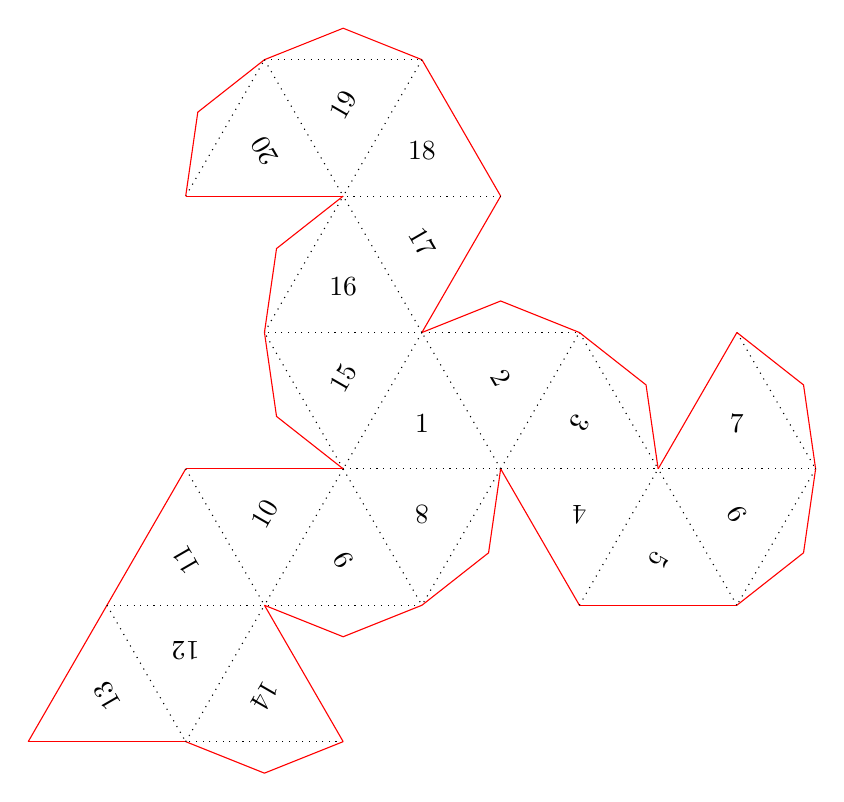
\begin{tikzpicture}[transform shape,every cut/.style=red,every fold/.style=dotted]
	\tikzfoldingicosahedron
	[folding line length=20mm,numbered faces];
\end{tikzpicture}
\clearpage
\begin{tikzpicture}[transform shape,every cut/.style=red,every fold/.style=dotted]
	\tikzfoldingtruncatedtetrahedron
	[folding line length=20mm,numbered faces];
\end{tikzpicture}
\clearpage
\begin{tikzpicture}[transform shape,every cut/.style=red,every fold/.style=dotted]
	\tikzfoldingcuboctahedron
	[folding line length=20mm,numbered faces];
\end{tikzpicture}
\clearpage
\begin{tikzpicture}[transform shape,every cut/.style=red,every fold/.style=dotted]
	\tikzfoldingtruncatedcube
	[folding line length=15mm,numbered faces];
\end{tikzpicture}
\clearpage
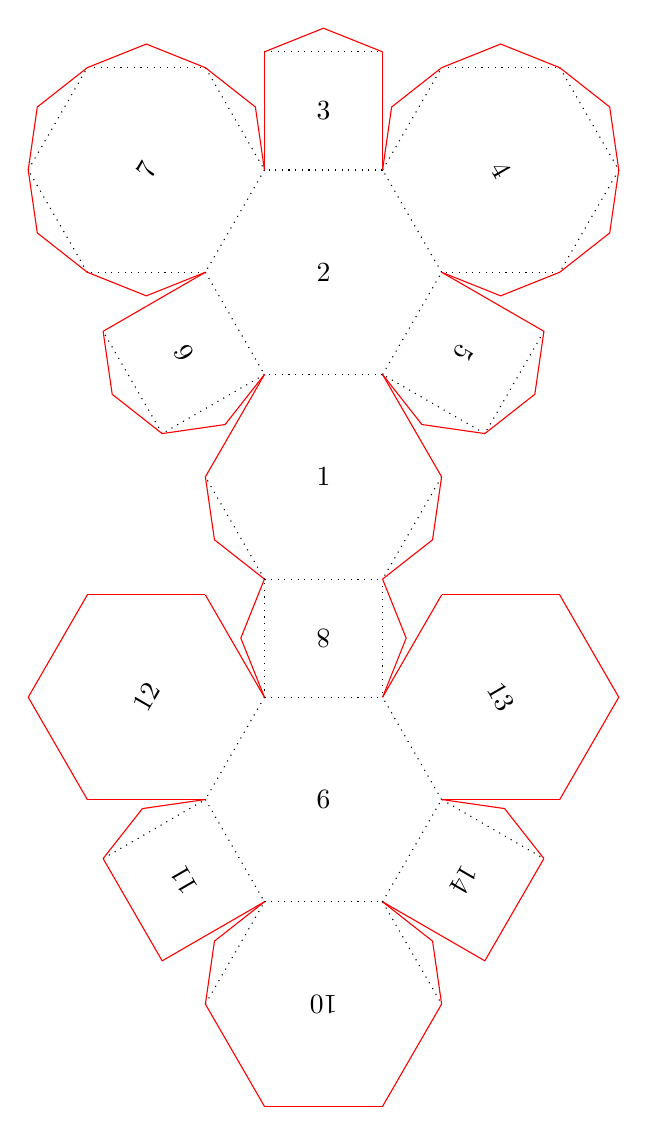
\begin{tikzpicture}[transform shape,every cut/.style=red,every fold/.style=dotted]
	\tikzfoldingtruncatedoctahedron
	[folding line length=15mm,numbered faces];
\end{tikzpicture}
\end{document}
